% Chapter 3

\chapter{Results} % Main chapter title
\label{Chapter3} % For referencing the chapter elsewhere, use \ref{Chapter3} 
\addtocontents{toc}{\setcounter{tocdepth}{1}}
\section{Assessment of GLUT1 inducible expression}
Previous results from the work of our laboratory showed that the GLUT1\textsuperscript{P485L} mutation leads to specific interaction with clathrins and internalization of the protein. In order to further investigate the role and functional effects of the mutation, we generated two Flp-In T-Rex HEK293 cell lines containing inducible BirA-FLAG epitope-tagged full length wild-type or mutant GLUT1 (Figure~\ref{fig:vectors}). 

To determine the optimal conditions for inducible expression, GLUT1 wild-type and mutant cells were grown in different concentrations of doxycycline for 24 hr and the expression of the GLUT1 protein was analyzed by Western blotting. The results showed that (Figure~\ref{fig:wb} A).
\begin{figure}[h]
\centering
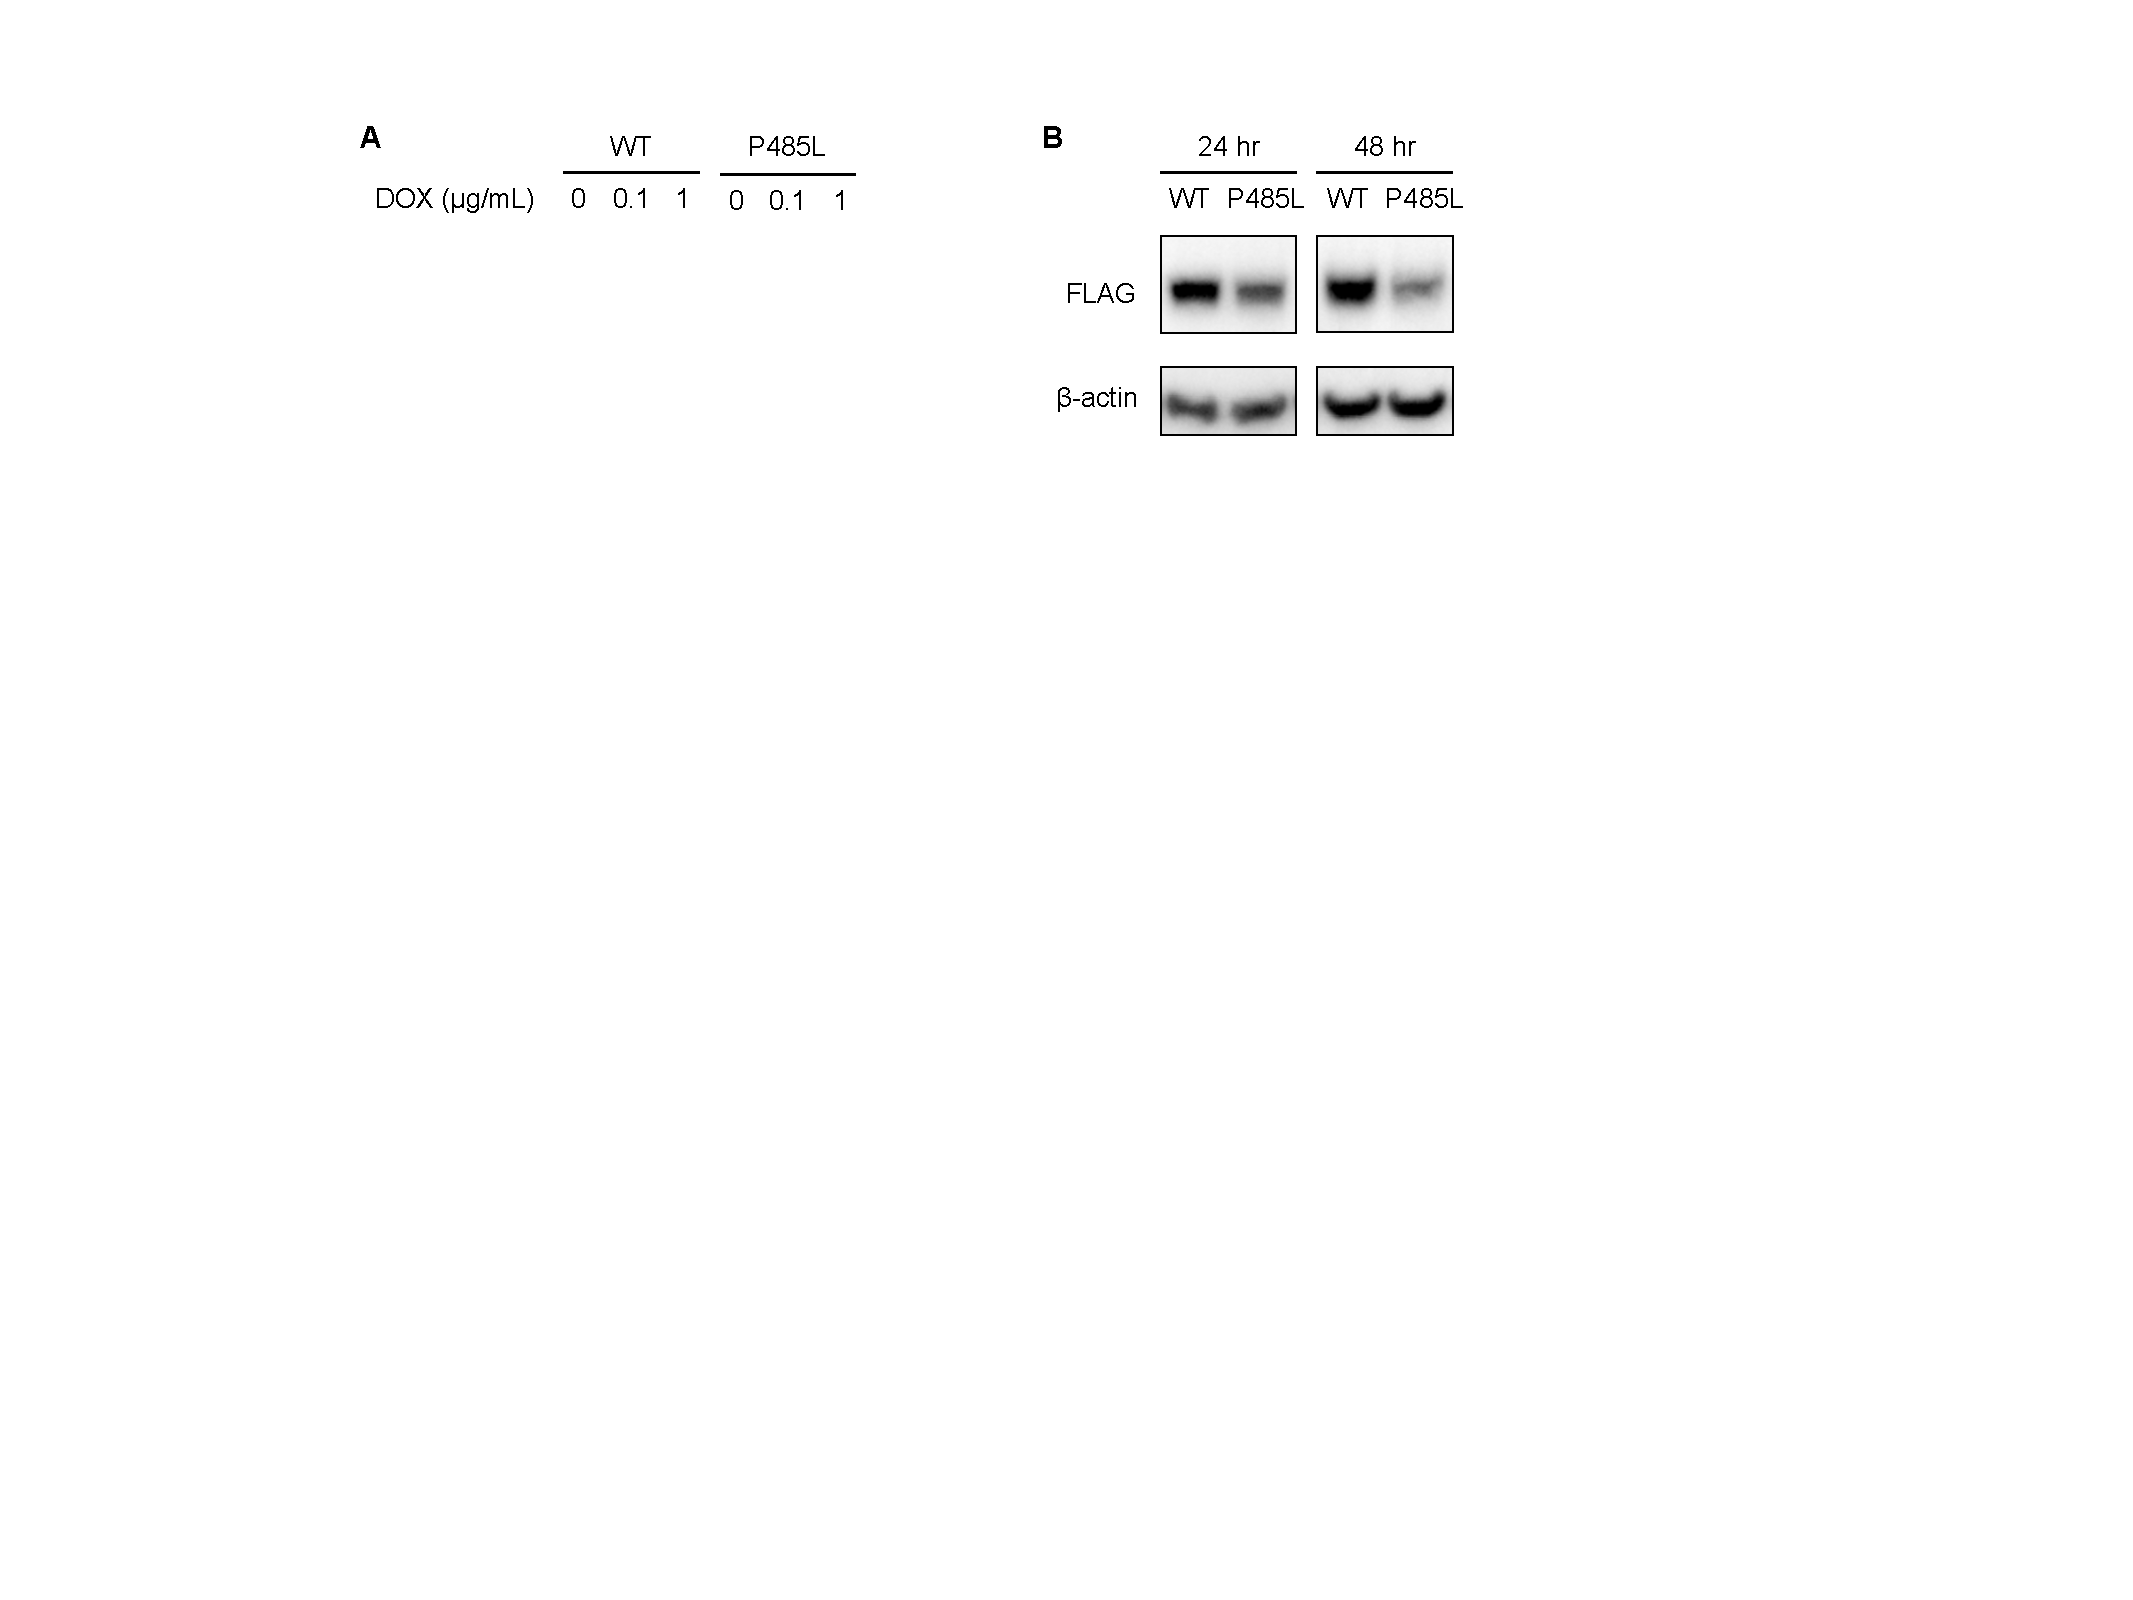
\includegraphics[scale=0.7]{Figures/WB}
\caption{The doxycycline-inducible expression of GLUT1 variants.}
\medskip
\small \raggedright
GLUT1 wild-type and mutant cells
\label{fig:wb}
\end{figure}

Two different induction times were tested

% leakiness in expression, microscopy picture?

In addition, the doxycycline-inducible expression of GLUT1 was confirmed by confocal immunofluorescence microscopy. GLUT1 wild-type and mutant cells were grown on coverslips and incubated in medium with or without doxycycline for 24 hr. Immunostaining was performed with monoclonal mouse anti-FLAG and Alexa 488-conjugated anti-mouse antibodies. A low level of GLUT1 expression was observed in a small fraction of uninduced wild-type cells (Figure~\ref{fig:IF} A).
\begin{figure}[h]
\centering
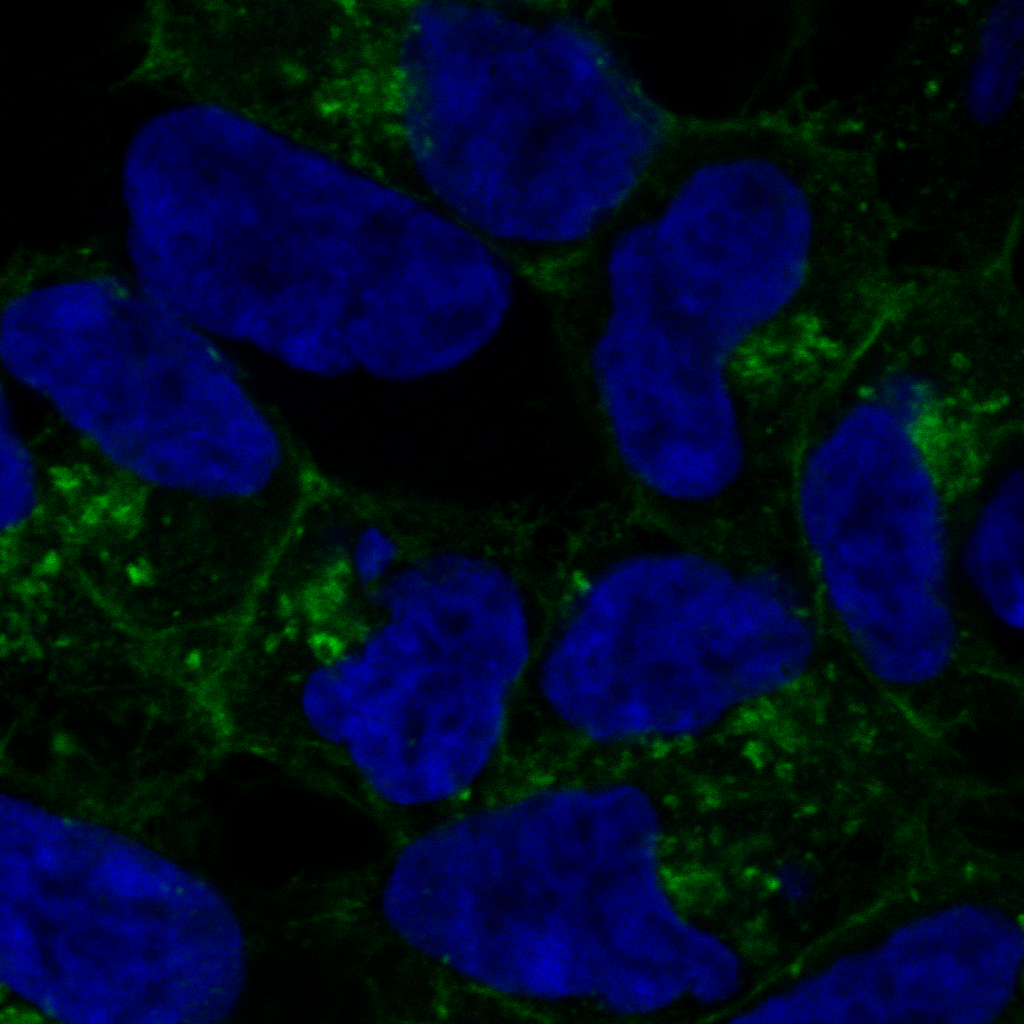
\includegraphics[scale=0.2]{Figures/induction_IF}
\caption{The inducible expression and localization of GLUT1 variants.}
\medskip
\small \raggedright
GLUT1 wild-type and mutant cells were cultured for 24 hr either in the absence or presence of 0.1 {}\textmu g/mL doxycycline. The expression of GLUT1 was assessed by immunofluorescence microscopy. A small subpopulation of uninduced wild-type cells showed weak expression of GLUT1 (A)
\label{fig:IF}
\end{figure}
%As expected, ARF localized to nucleolar regions (the compact circular regions of higher intensity as pointed by the arrow in panel A) while HA-RBP1 demonstrated strong nuclear localization with nucleolar exclusion, as shown by the dark nucleolar regions in panel B. Panel C confirms that RBP2 is localized exclusively to the nucleus. Panel D illustrates that the rabbit polyclonal ?-RBP2 antibody cannot be used in immunofluorescence because of the high amount of non-specific background signal it produces. Trials were done at various dilutions but all were negative and produced the same non-specific noise (data not shown). 
\section{Proximity labeling of GLUT1 variants}

\section{Co-localization study of GLUT1 variants}

%----------------------------------------------------------------------------------------
% Define some commands to keep the formatting separated from the content 
